\documentclass[13pt]{book}              % Book class in 11 points

\title{\bf Manual de usuario}    % Supply information
\author{
  Ismael Tobar Garcia     
  \\[3ex]
  D. Alvar Arnáiz González
  \\[3ex]
  Dr. José Francisco Diez Pastor
  \\[3ex]
}
\date{\today}                           
\newpage

% Castellano
\usepackage[spanish]{babel}
\selectlanguage{spanish}
\usepackage[utf8]{inputenc}
\usepackage{placeins}
\usepackage{caption}
\usepackage{subcaption}
\usepackage[linesnumbered,ruled,vlined,spanish]{algorithm2e}

\RequirePackage{booktabs}
\RequirePackage[table]{xcolor}
\RequirePackage{xtab}
\RequirePackage{multirow}

%\usepackage{sectsty}
%\sectionfont{\LARGE}

\usepackage{titlesec}
\titleformat*{\section}{\Huge\bfseries}
\titleformat*{\subsection}{\huge\bfseries\sffamily}


% Links
\usepackage[colorlinks]{hyperref}
\hypersetup{
	allcolors = {red}
}

% Ecuaciones
\usepackage{amsmath}

% Rutas de fichero / paquete
\newcommand{\ruta}[1]{{\sffamily #1}}

% Imagenes
\usepackage{graphicx}
\newcommand{\imagen}[2]{
	\begin{figure}[!h]
		\centering
		\includegraphics[width=0.9\textwidth]{#1}
		\caption{#2}\label{fig:#1}
	\end{figure}
	\FloatBarrier
}

\newcommand{\imagenflotante}[2]{
	\begin{figure}%[!h]
		\centering
		\includegraphics[width=0.9\textwidth]{#1}
		\caption{#2}\label{fig:#1}
	\end{figure}
}

\graphicspath{ {./img/} }



\begin{document}                       
\maketitle         
\cleardoublepage                   
\tableofcontents                       
\newpage



\section{Manual del usuario}
{ \huge

Una vez tengamos todo bien configurado y la aplicación ejecute correctamente deberíamos tener esta ventana inicial.

\begin{figure}[h]
\centering
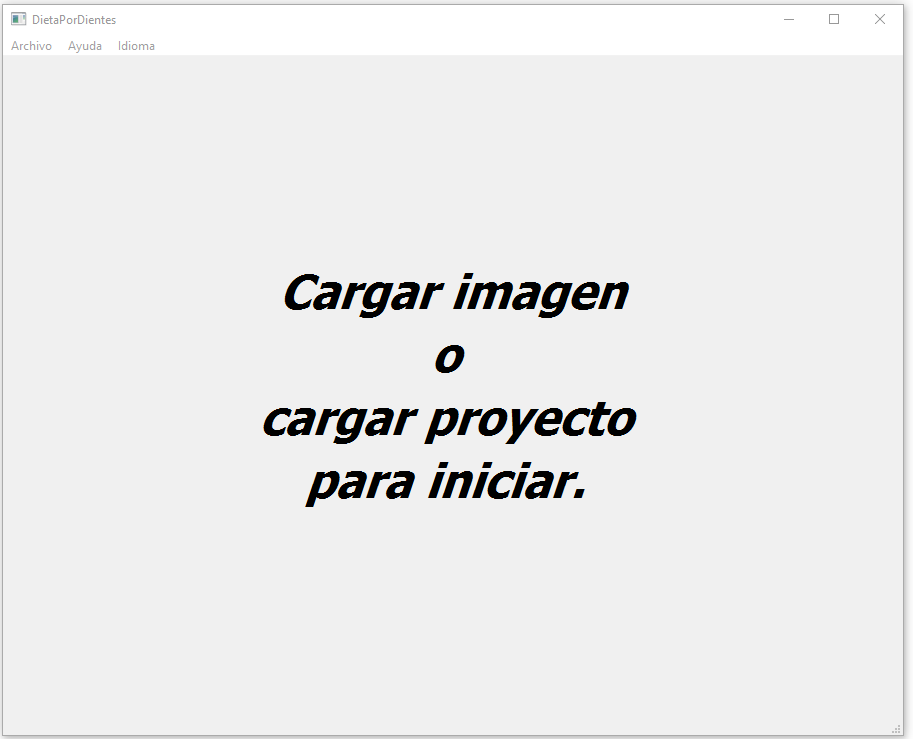
\includegraphics[width=.99\textwidth]{VentanaInicial}
\caption{Ventana inicial de la aplicación}
\label{fig:E.1}
\end{figure}
Una vez llegados a este punto tendremos varias opciones para editar o calculas las estrías de una imagen, dependiendo si esta en blanco o ya pintada tendremos las siguientes opciones:

\begin{itemize}
	\item Abrir imagen \ref{modo:1}:

	\item Cargar proyecto \ref{modo:2}:
	
\end{itemize}


\label{modo:1}
\subsection{Abrir imagen}
En esta sección se explicara como cargar una imagen en nuestra aplicación, para empezar un proyecto desde cero.

Deberemos seleccionar la opción de Archivo  $>$ Nuevo Proyecto. Como se puede ver en la imagen \ref{fig:abrirPro}

\begin{figure}[h]
\centering
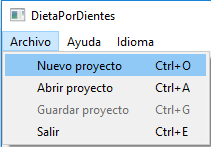
\includegraphics[width=.50\textwidth]{AbrirImagen}
\caption{Opción para cargar una imagen}
\label{fig:abrirPro}
\end{figure}

Una vez que clicamos en este punto se nos muestra una ventana de elegir ficheros en el cual debemos explorar hasta la carpeta donde estén las imágenes que queremos analizar. Como podemos observar en la figura \ref{fig:abrirPaso2}

\begin{figure}[h]
\centering
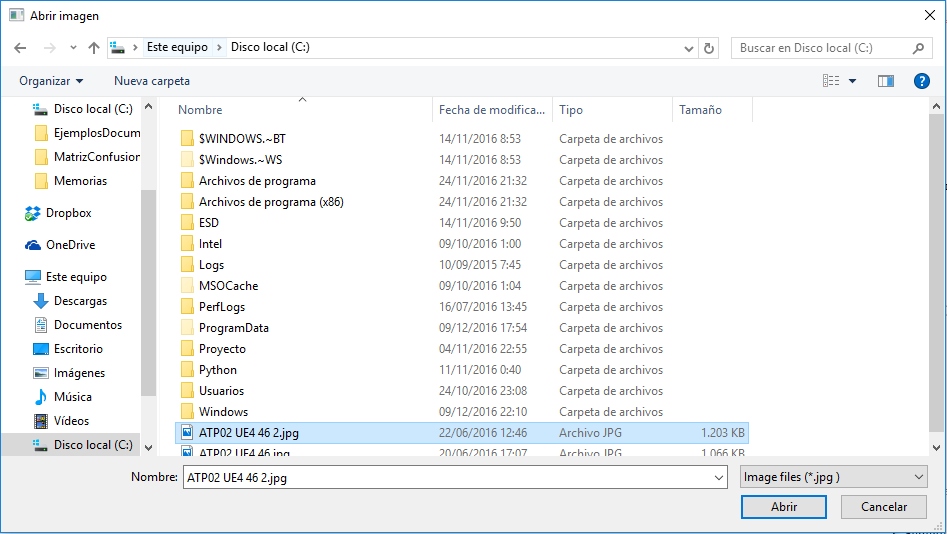
\includegraphics[width=.99\textwidth]{AbrirPaso2}
\caption{Seleccionador de ficheros}
\label{fig:abrirPaso2}
\end{figure}

Una vez seleccionado deberemos dar a aceptar si hemos seleccionado la imagen que queremos evaluar.
Dependiendo de la imagen que hemos abierto pueden pasar dos cosas, uno \ref{fig:opcion1}, que la imagen abierta este pintada, dos \ref{fig:opcion2}, que la imagen abierta no este pintada. Dependiendo de esto tendremos estas dos ventanas, como se muestra en la figura.


\begin{figure}
	\begin{subfigure}[c]{.5\linewidth}
	\centering\large 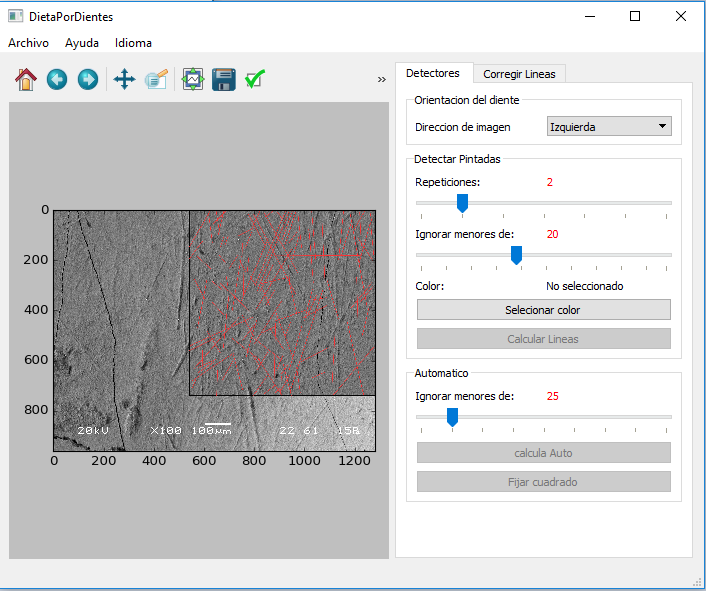
\includegraphics[width=.9\textwidth]{opcion1}
	\caption{Opcion con lineas pintadas.}\label{fig:opcion1}
	\end{subfigure}%
	\begin{subfigure}[c]{.5\linewidth}
	\centering\large 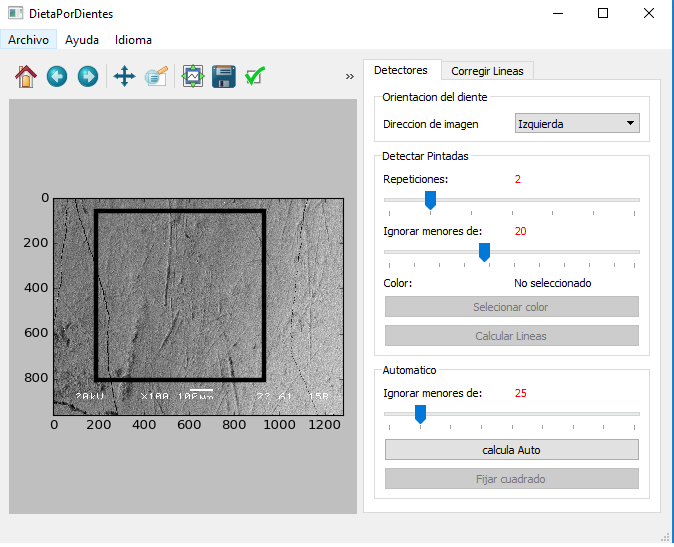
\includegraphics[width=.9\textwidth]{opcion2}
	\caption{Opcion con lineas sin pintar.}\label{fig:opcion2}
	\end{subfigure}%
\end{figure}




\label{modo:2}
\subsection{Cargar proyecto}
En esta sección se explicara como cargar un proyecto en nuestra aplicación, para continuar un proyecto ya empezado.

Deberemos seleccionar la opción de Archivo  $>$ Abrir Proyecto. Como se puede ver en la figura \ref{fig:cargarPro}


\begin{figure}[h]
\centering
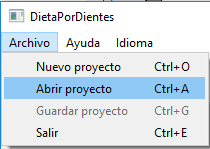
\includegraphics[width=.50\textwidth]{CargarProyecto}
\caption{Opción para abrir un proyecto.}
\label{fig:cargarPro}
\end{figure}

Una vez que hacemos clic sobre la opción anteriormente mencionada ahora debemos seleccionar la carpeta donde estará contenido todos los ficheros del proyecto, como podemos observar en la siguiente figura \ref{fig:selecCargarPro}. y una vez seleccionado el directorio que contiene los ficheros del proyecto damos a <<Abrir carpeta>> para cargar el proyecto. 



\begin{figure}[h]
\centering
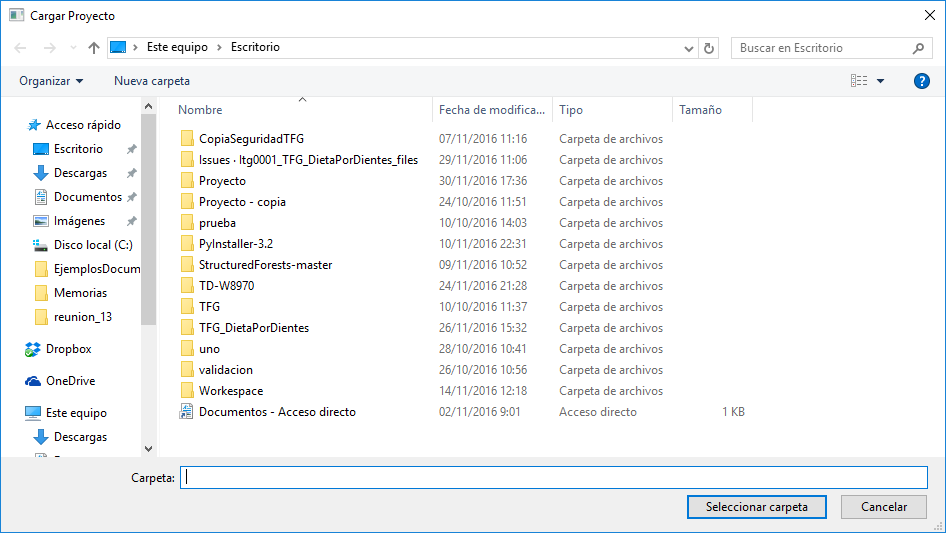
\includegraphics[width=.99\textwidth]{selecCargarPro}
\caption{Opción para abrir un proyecto.}
\label{fig:selecCargarPro}
\end{figure}

Una vez abierto el proyecto tendremos la imagen en blanco y negro junto con sus estrías guardadas que estarán pintadas sobre la imagen, como podemos observar en la figura \ref{fig:proyectoAbierto}.


\begin{figure}[h]
\centering
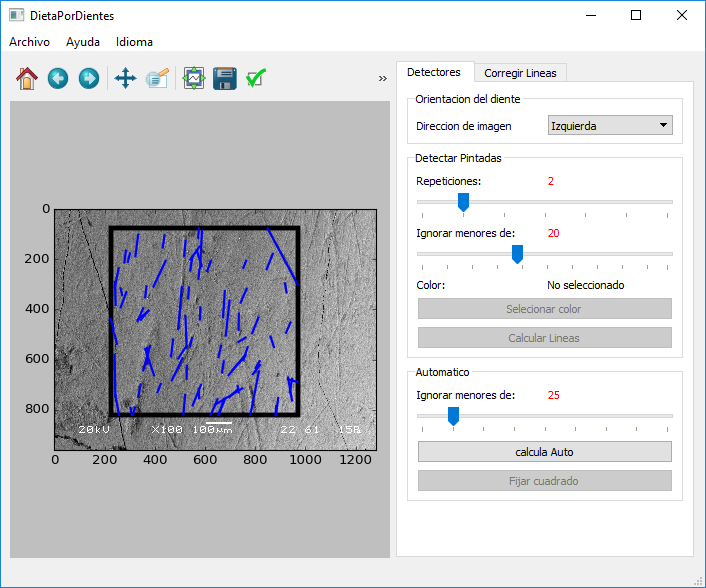
\includegraphics[width=.99\textwidth]{proyectoAbierto}
\caption{Como se muestra un proyecto cargado o abierto.}
\label{fig:proyectoAbierto}
\end{figure}

\label{modo:idioma}
\subsection{Cambiar idioma}
Para cambiar el idioma de la aplicación deberemos seleccionar en el menú principal Idioma $>$ Una de las dos opciones, como podemos observar en la figura \ref{fig:camb}, hemos optado por cambiar el idioma de la aplicación y que perduren los cambios realizados en el fichero de configuración por lo que nos va a pedir reiniciar la aplicación, si tenemos algo abierto nos preguntara si queremos guardar los cambios o no.

\begin{figure}[h]
\centering
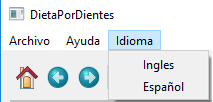
\includegraphics[width=.55\textwidth]{CambiarIdioma}
\caption{Como cambiar el idioma.}
\label{fig:camb}
\end{figure}

\subsection{Modo semi-automático para lineas pintadas}

Este modo solamente podrá ser usado cuando dispongamos de una imagen que tenga las estrías pintadas sobre ella y estas estén contenidas dentro de un cuadrado que delimite su área, como podemos observar en la figura \ref{fig:semiAutoCorrecto}.



\begin{figure}[h]
\centering
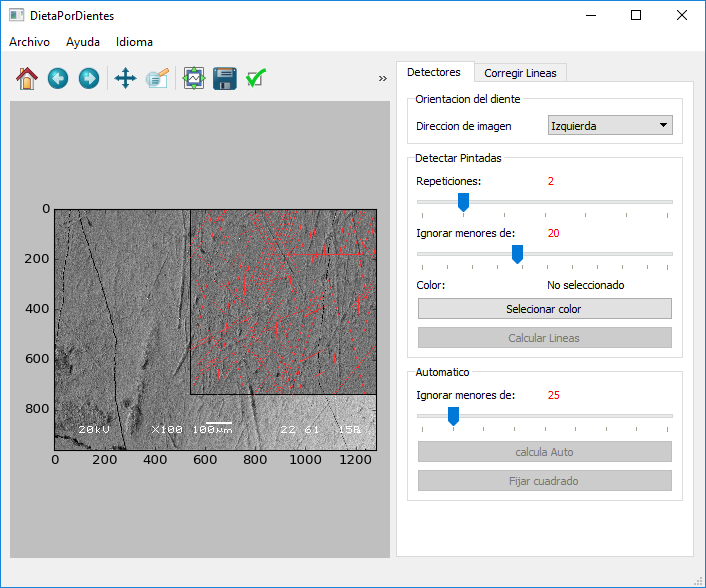
\includegraphics[width=.99\textwidth]{semiAutoCorrecto}
\caption{Imagen valida para detección de estrías modo semiautomático.}
\label{fig:semiAutoCorrecto}
\end{figure}

Una vez que tengamos una imagen con las estrías pintadas cargada y valida como mostramos en la figura, procederemos a seleccionar su orientación, como muestra en la siguiente figura \ref{fig:selOrientacion}.

\begin{figure}[h]
\centering
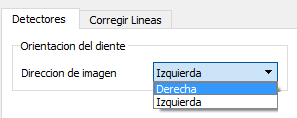
\includegraphics[width=.55\textwidth]{selOrientacion}
\caption{Selección de la orientación de la imagen.}
\label{fig:selOrientacion}
\end{figure}

A continuación deberemos seleccionar tanto el numero de repeticiones del algoritmo para la obtención de los segmentos pintados <<Cuanto mayor número de ellos mas tiempo tardara>>, la longitud mínima que debe ignorar el algoritmo para no detectar segmentos muy pequeños. Como podemos observar en la figura \ref{fig:opcionesAlg}.

\begin{figure}[h]
\centering
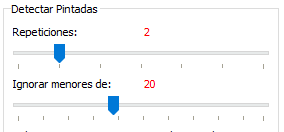
\includegraphics[width=.55\textwidth]{opcionesAlg}
\caption{Selección de las opciones disponibles para este modo.}
\label{fig:opcionesAlg}
\end{figure}

Finalmente para nos quedaría la opción mas importante que sin ella el algoritmo no podrá ser ejecutado. Es seleccionar el color del que estén pintadas las lineas, para ello deberemos clicar sobre el botón <<Seleccionar color>>, como podemos observar en la figura \ref{fig:selecionarColorP1} y después de clicar sobre el este se desactivara como podemos observar en la figura \ref{fig:selecionarColorP2}.
Las estrías pintadas aveces pueden ser muy finas y no seremos capaces de clicar sobre esos pixeles por lo que en este caso deberemos ampliar la imagen en una región que contenga estrías pintadas, para ampliar debemos seleccionar el botón de ampliar y dibujar un rectángulo sobre la imagen con el clic derecho pulsado,como podemos observar en la figura \ref{fig:selecionarColorP3}.
Una vez seleccionado el color correctamente este pintada el label de color actual y también se activara el botón de calcular las lineas, como podemos observar en la figura \ref{fig:selecionarColorP4}.



\begin{figure}
	\begin{subfigure}[c]{.5\linewidth}
	\centering\large 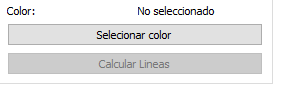
\includegraphics[width=.9\textwidth]{selecionarColorP1}
	\caption{Selección del color en el que estén las estrías pintadas.}\label{fig:selecionarColorP1}
	\end{subfigure}%
	\begin{subfigure}[c]{.5\linewidth}
	\centering\large 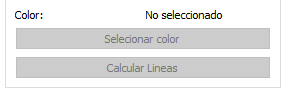
\includegraphics[width=.9\textwidth]{selecionarColorP2}
	\caption{Después de clicar sobre el.}
	\label{fig:selecionarColorP2}
	\end{subfigure}%
	
	\begin{subfigure}[c]{.5\linewidth}
	\centering\large 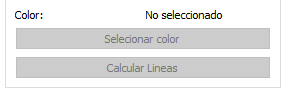
\includegraphics[width=.9\textwidth]{selecionarColorP2}
	\caption{Ampliar región.}
	\label{fig:selecionarColorP3}
	\end{subfigure}%
	\begin{subfigure}[c]{.5\linewidth}
	\centering\large 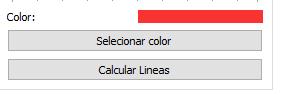
\includegraphics[width=.9\textwidth]{selecionarColorP4}
	\caption{Después de seleccionar correctamente el color.}
	\label{fig:selecionarColorP4}
	\end{subfigure}%
\end{figure}

Para finalizar una vez que cliquemos en el botón de calcular lineas ya podremos añadir estrías nuevas, eliminar algunos segmentos, borrar todos o guardar los datos del proyecto para calcular las estadísticas de las estrías.


\subsection{Modo manual}
Después de cargar una imagen ya sea pintada o sin pintar deberemos abrir una imagen como indica el apartado \ref{modo:1} o abrir un proyecto tal y como indican el apartado \ref{modo:2}.
Una vez que tengamos la imagen o el proyecto cargado podremos pintar nuevas estrías en la imagen siguiendo los siguientes pasos.

\begin{itemize}
\item Pulsaremos el botón de corregir lineas, como muestra la siguiente figura \ref{fig:CorregirPaso1}.

\item Una vez pulsado deberemos seleccionar dos puntos, uno el inicio y el segundo, el final del segmento que queremos añadir. 
Dentro del recuadro de la región factible que esta delimitada por un recuadro negro, como se muestra en las figuras \ref{fig:punto1} y \ref{fig:punto2}, ahora solo nos quedara añadir el segmento a la tabla como muestra la figura \ref{fig:anadirsegment}.
\end{itemize}

\begin{figure}
	\begin{subfigure}[c]{.5\linewidth}
	\centering\large 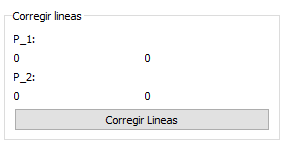
\includegraphics[width=.9\textwidth]{CorregirPaso1}
	\caption{Activar el modo de corregir o añadir un segmento.}\label{fig:CorregirPaso1}
	\end{subfigure}%
	\begin{subfigure}[c]{.5\linewidth}
	\centering\large 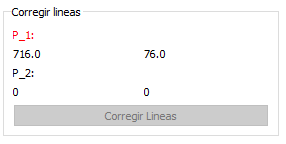
\includegraphics[width=.9\textwidth]{punto1}
	\caption{Primer punto seleccionado.}\label{fig:punto1}
	\end{subfigure}%
	
	\begin{subfigure}[c]{.5\linewidth}
	\centering\large 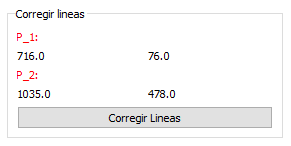
\includegraphics[width=.9\textwidth]{punto2}
	\caption{Segundo punto seleccionado.}\label{fig:punto2}
	\end{subfigure}%
	\begin{subfigure}[c]{.5\linewidth}
	\centering\large 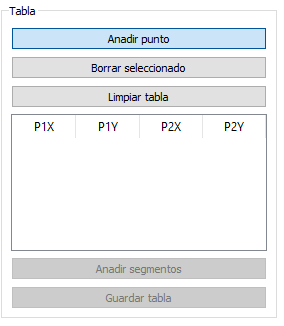
\includegraphics[width=.9\textwidth]{anadirsegment}
	\caption{Añadir segmento.}\label{fig:anadirsegment}
	\end{subfigure}%
\end{figure}

	
Para los demás pasos no hace falta explicación ya que sus respectivos botones dicen claramente que funciones desempeñan.	
	
\subsection{Modo automático}
Después de cargar una imagen sin pintar deberemos abrir una imagen como indica el apartado \ref{modo:1} o abrir un proyecto tal y como indica el apartado \ref{modo:2}.

Una vez que tengamos la imagen o el proyecto cargado, podremos configurar el modo automático, lo primero sera asignar la orientación de la imagen, como podemos ver en la figura \ref{fig:selOrientacion}, también deberemos seleccionar la longitud mínima de corte que ignorara el algoritmo automático, como podemos observar en la figura \ref{fig:selTam}.

\begin{figure}[h]
\centering
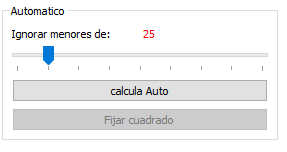
\includegraphics[width=.55\textwidth]{selTam}
\caption{Selección de la longitud mínima de corte.}
\label{fig:selTam}
\end{figure}

Una vez seleccionado el tamaño mínimo de corte podremos ejecutar el algoritmo clicando el botón de calar automático obteniendo el resultado mostrado en la figura \ref{fig:CalculadasAuto} y podremos mover el recuadro del área con el que nos queremos quedar a la región de interés que consideremos apropiada.

\begin{figure}[h]
\centering
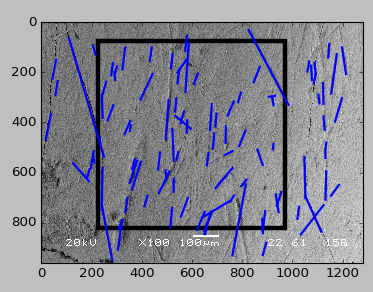
\includegraphics[width=.55\textwidth]{CalculadasAuto}
\caption{Selección de la longitud mínima de corte.}
\label{fig:CalculadasAuto}
\end{figure}

una vez que la situemos donde mayor densidad de estrías haya detectado, la fijaremos e ignorara las que se queden por fuera de la región, como podemos observar en la figura \ref{fig:automati}.

\begin{figure}[h]
\centering
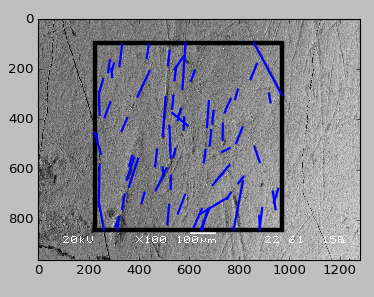
\includegraphics[width=.55\textwidth]{automati}
\caption{Selección de la longitud mínima de corte.}
\label{fig:automati}
\end{figure}

Pasado este punto en la pestaña de corregir lineas quedaran añadidas todas aquellas que ha detectado el algoritmo y hemos encuadrado en la región factible, de estas lineas podremos obtener tanto estadísticas como un proyecto para editar mas adelante. Guardando el proyecto con el botón para dicha función.

\subsection{Guardar proyecto}

En este apartado vamos a explicar como guardar un proyecto una vez que hayamos abierto o cargado una imagen, calculado las estrías con el modo semiautomático o por el automático, y la tabla este rellenada con estas. 
Si el proyecto es cargado de uno ya existente, no tener abiertas las estadísticas en Excel porque sino no funcionara la operación de guardar, esto sera transparente al usuario porque dejara los ficheros como estaban antes, no los modificara, e informara al usuario de que no han sido guardados. 

Podemos usar tanto el botón de guardar que aparece en la pestaña dos \ref{fig:BotonGuarPesta} como el botón del menú principal que aparece en la figura \ref{fig:BotonGuar}

\begin{figure}
	\begin{subfigure}[c]{.5\linewidth}
	\centering\large 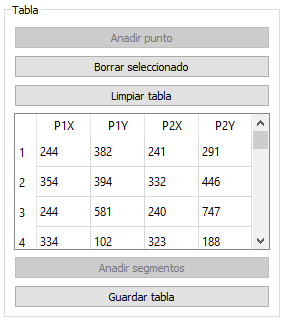
\includegraphics[width=.9\textwidth]{BotonGuarPesta}
	\caption{Boton de guardar en la pestaña dos.}\label{fig:BotonGuarPesta}
	\end{subfigure}%
	\begin{subfigure}[c]{.5\linewidth}
	\centering\large 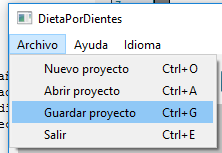
\includegraphics[width=.9\textwidth]{BotonGuar}
	\caption{Boton de guardar en el menu principal.}\label{fig:BotonGuar}
	\end{subfigure}%
\end{figure}
}
\end{document}                         
